All reported runs passed the split and research-validity gates.

\subsection{Target-Performer Exposure}

Target-performer exposure increased fixed-test accuracy in all 20 architecture--performer comparisons. The mean increase was 0.164, the median was 0.154, and the range was 0.024--0.304. Averaged across models and seeds, H01--H04 improved from 0.836, 0.739, 0.905, and 0.694 under Protocol A to 0.953, 0.956, 0.973, and 0.949 under Protocol B. Overall mean accuracy increased from 0.794 to 0.958. Fig.~\ref{fig:exposure_gap} shows the same result performer by performer.

\begin{figure}[tbp]
\centering
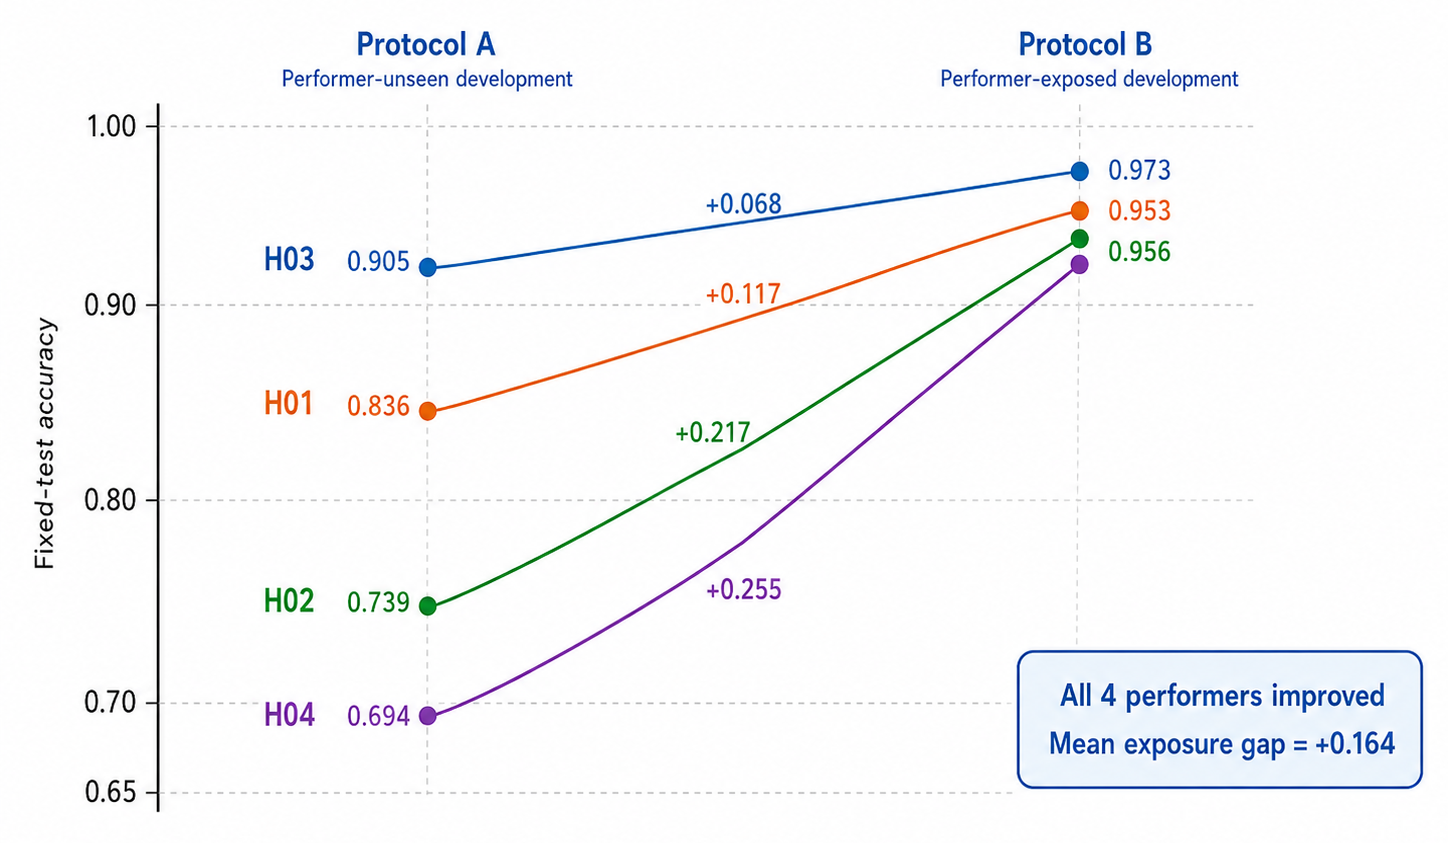
\includegraphics[width=0.84\linewidth]{Figures/Figure3_exposure_gap.png}
\caption{Fixed-test accuracy under performer-unseen and performer-exposed development, averaged over five architectures and three seeds. All four target performers improved; the mean exposure gap was 0.164.}
\label{fig:exposure_gap}
\end{figure}

This gap exceeded the 0.116 range among Hòa Đê architecture means, though the two are not statistically equivalent effect measures and we do not treat them as such. Our claim is descriptive: within this dataset and this configuration set, the protocol difference was larger than the spread among model-family means. One point of interpretation matters. Protocol B exposes the target performer to optimization and to validation-based selection at once, so what we measured is performer exposure across model development as a whole, not training-only leakage.

\subsection{Hòa Đê Held-Out-Performer Results}

The Hòa Đê reference accuracies were 0.143 for uniform chance, 0.146 for the majority class, 0.552 for nearest centroid, and 0.719 for 1-NN.

\begin{table}[htbp]
\centering
\caption{Hòa Đê held-out-performer accuracy. Cells are means over three seeds; SD is computed across the four performer means.}
\label{tab:hoa_de}
\small
\setlength{\tabcolsep}{3.8pt}
\renewcommand{\arraystretch}{1.08}
\begin{tabularx}{\linewidth}{L c c c c c c}
\toprule
\textbf{Model} & \textbf{H01} & \textbf{H02} & \textbf{H03} & \textbf{H04} & \textbf{Mean} & \textbf{SD} \\
\midrule
HandGCN & 0.941 & 0.823 & 0.971 & 0.775 & 0.878 & 0.094 \\
CNN & 0.829 & 0.748 & 0.946 & 0.657 & 0.795 & 0.123 \\
TCN & 0.846 & 0.701 & 0.898 & 0.641 & 0.772 & 0.120 \\
LSTM & 0.804 & 0.736 & 0.924 & 0.600 & 0.766 & 0.135 \\
BiGRU+Attn & 0.776 & 0.771 & 0.838 & 0.663 & 0.762 & 0.073 \\
\bottomrule
\end{tabularx}
\end{table}

\begin{figure}[tbp]
\centering
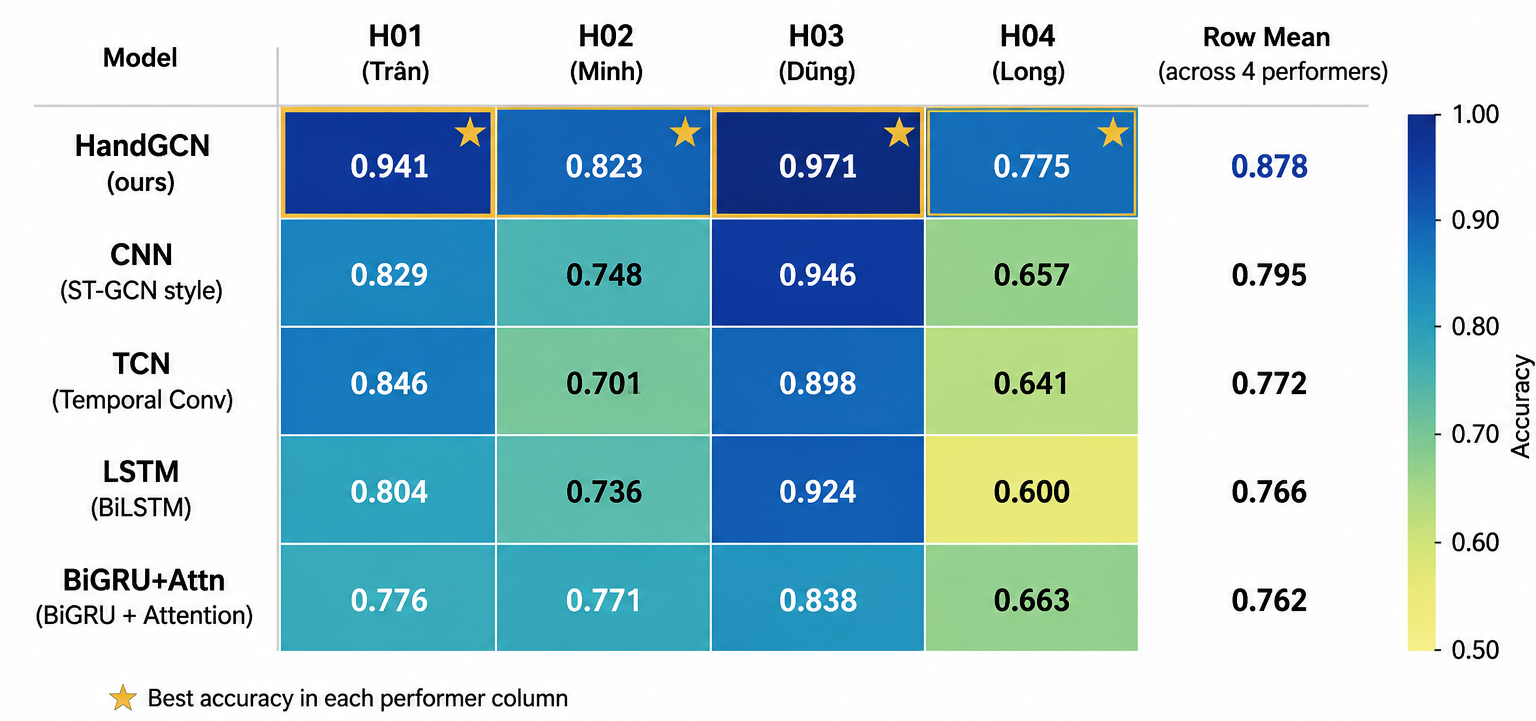
\includegraphics[width=0.95\linewidth]{Figures/Figure4_hoa_de_heatmap.png}
\caption{Held-out-performer accuracy on the Hòa Đê profile, per architecture
and per target performer, with row means across the four performers. Stars
mark the best architecture in each performer column. The same values appear
in Table~\ref{tab:hoa_de}.}
\label{fig:hoa_de_heatmap}
\end{figure}

Table~\ref{tab:hoa_de} reports the full fold-by-fold results, and
Fig.~\ref{fig:hoa_de_heatmap} shows the same matrix as a heatmap, where the
column-wise structure is easier to read off. HandGCN ranked first on all four folds and took the highest mean accuracy, 0.878, with CNN second at 0.795 and a spread of 0.116 across architecture means. The margins behind that sweep are uneven: 0.095, 0.052, 0.025, and 0.112 over the runner-up at H01 through H04. The narrowest of them, 0.025 over CNN at H03, is thin enough that we present the sweep as a description of these three seeds rather than as a stable property of the architecture. Averaged across models, H01--H04 scored 0.839, 0.756, 0.916, and 0.667, a spread of 0.249. Performer-level variation was thus descriptively larger than architecture-level variation. H03 proved easiest and H04 hardest; H03 is also the originating Deaf performer, but with exactly one originator in the profile we cannot separate that role from anything else about them, and we draw no originator effect from it.

\subsection{Fingerspelling Results}

\begin{table}[htbp]
\centering
\caption{Accuracy on the 23-class fingerspelling subset, averaged over three seeds.}
\label{tab:fingerspelling}
\small
\setlength{\tabcolsep}{7pt}
\renewcommand{\arraystretch}{1.08}
\begin{tabular}{lccc}
\toprule
\textbf{Model} & \textbf{F01} & \textbf{F02} & \textbf{Mean} \\
\midrule
BiGRU+Attn & 0.885 & 0.752 & 0.819 \\
HandGCN & 0.829 & 0.774 & 0.802 \\
TCN & 0.866 & 0.703 & 0.785 \\
LSTM & 0.854 & 0.695 & 0.775 \\
CNN & 0.840 & 0.697 & 0.769 \\
\bottomrule
\end{tabular}
\end{table}

In Table~\ref{tab:fingerspelling}, BiGRU+Attn took the highest two-fold mean and HandGCN came second, but the two folds disagree about which is better: BiGRU+Attn wins F01 and HandGCN wins F02. The architecture means span only 0.050, and several models differ more than that between the two performers alone. Two folds that contradict each other, separated by less than the within-model performer gap, do not support a stable fingerspelling ranking, and we do not report one.

\subsection{Reproducibility Evidence}

Repeating commit \texttt{28f0393} for HandGCN, CNN, and TCN under one fixed environment, seed, and split reproduced bit-identical model states, predictions, and metrics, across 24 checks per model. The cross-revision comparison came out weaker: over 90 paired configurations predictions were unchanged and metrics agreed to four decimals, but some HandGCN parameters differed by roughly $10^{-6}$.

We therefore establish same-code determinism only for that commit, those three architectures, and that one RTX 3050 environment, and we claim nothing past it. The cross-revision result we read as behavioral stability, not as byte-identical models.